\documentclass[border={0.1cm 0.1cm 0.1cm 0.1cm}]{standalone}  %E,S,W,N

\usepackage{amssymb}
\usepackage{amsmath}
\usepackage{tikz}
\usetikzlibrary{calc}	%for centerarc

\def\centerarc[#1](#2)(#3:#4:#5) {\draw[#1] ($(#2)+({#5*cos(#3)},{#5*sin(#3)})$) arc (#3:#4:#5);}

%Diagram of the Possibilities in Any Negotiation, from Garin, Grant, Saunders - A Negotiations Model: a Form for Private and Public Sector Bargaining (1973)

\begin{document}
	
	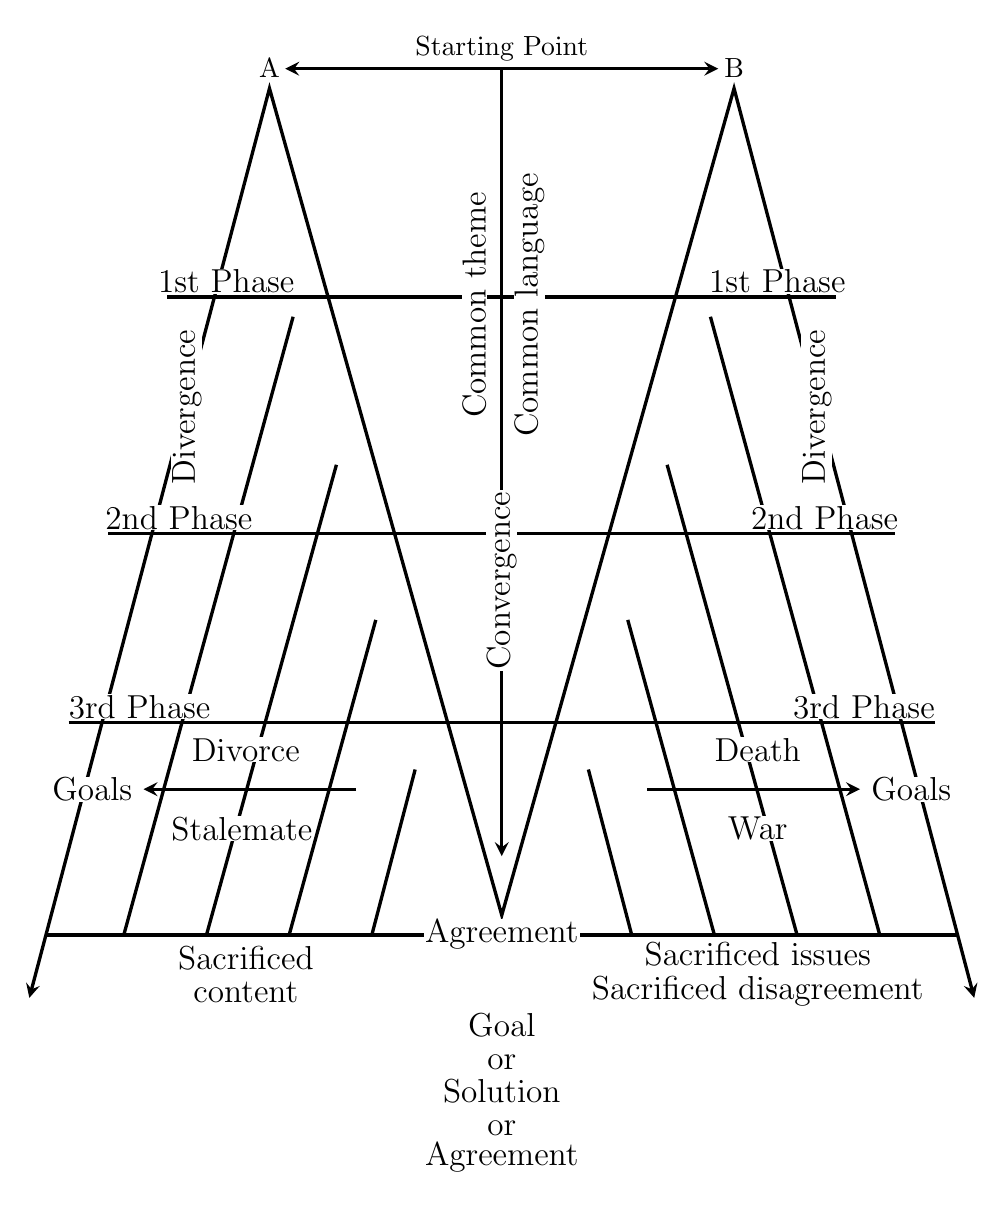
\begin{tikzpicture}[very thick]
	%MAIN LINES
	\draw[<->,>=stealth] (-2.75,11)--(2.75,11);
	\draw[->,>=stealth] (0,11)--(0,1);
	\draw[<->,>=stealth] (-6,-0.8)--(-2.95,10.75)--(0,0.25)--(2.95,10.75)--(6,-0.8);
	%
	\draw (-4.25,8.1)--(4.25,8.1);
	\draw (-5.0,5.1)--(5.0,5.1);
	\draw (-5.5,2.7)--(5.5,2.7);
	\draw (-5.8,0)--(5.8,0);
	%
	\centerarc[](-6.9,0.65)(82:-47:6.5)
	\centerarc[](6.9,0.65)(98:227:6.5)
	
	%DIAGONAL LINES
	\draw (-4.8,0)--(-2.65,7.85);		\draw (4.8,0)--(2.65,7.85);
	\draw (-3.75,0)--(-2.1,5.97);		\draw (3.75,0)--(2.1,5.97);
	\draw (-2.7,0)--(-1.6,4);			\draw (2.7,0)--(1.6,4);
	\draw (-1.65,0)--(-1.1,2.1);		\draw (1.65,0)--(1.1,2.1);
	%
	\draw[->,>=stealth] (-1.85,1.85)--(-4.55,1.85);
	\draw[->,>=stealth] (1.85,1.85)--(4.55,1.85);
	\node[fill=white,inner sep=0.4pt] at (-5.2,1.85) {\large Goals};
	\node[fill=white,inner sep=0.4pt] at (5.2,1.85) {\large Goals};
	\node[fill=white,inner sep=0.4pt] at (-3.25,2.35) {\large Divorce};
	\node[fill=white,inner sep=0.4pt] at (-3.3,1.35) {\large Stalemate};
	\node[fill=white,inner sep=0.4pt] at (3.25,2.35) {\large Death};
	\node[fill=white,inner sep=0.4pt] at (3.25,1.35) {\large War};
	
	%LABELS
	\node at (0,11.25) {Starting Point};
	\node[above] at (-2.95,10.75) {A};
	\node[above] at (2.95,10.75) {B};
	\node[fill=white,inner sep=0.4pt] at (-0.35,8) {\rotatebox{90}{\large Common theme}};
	\node[fill=white,inner sep=0.2pt] at (0.35,8) {\rotatebox{90}{\large Common language}};
	\node[fill=white,inner sep=0.4pt] at (0,4.5) {\rotatebox{90}{\large Convergence}};
	\node[fill=white,inner sep=0.4pt] at (-4,6.7) {\rotatebox{90}{\large Divergence}};
	\node[fill=white,inner sep=0.4pt] at (4,6.7) {\rotatebox{90}{\large Divergence}};
	%
	\node[fill=white,inner sep=0.4pt] at (-3.5,8.3) {\large 1st Phase};
	\node[fill=white,inner sep=0.4pt] at (3.5,8.3) {\large 1st Phase};
	\node[fill=white,inner sep=0.4pt] at (-4.1,5.3) {\large 2nd Phase};
	\node[fill=white,inner sep=0.4pt] at (4.1,5.3) {\large 2nd Phase};
	\node[fill=white,inner sep=0.4pt] at (-4.6,2.9) {\large 3rd Phase};
	\node[fill=white,inner sep=0.4pt] at (4.6,2.9) {\large 3rd Phase};
	\node[fill=white,inner sep=0.4pt] at (0,0) {\large Agreement};
	%
	\node[align=center] at (-3.25,-0.5) {\large Sacrificed \\\large content};
	\node[align=center] at (3.25,-0.5) {\large Sacrificed issues \\\large Sacrificed disagreement};
	\node[align=center] at (0,-2) {\large Goal \\\large or \\\large Solution \\\large or \\[-0.5mm]\large Agreement};
	\end{tikzpicture}
	
\end{document}